\documentclass[12pt,fleqn]{article}\usepackage{../common}
\begin{document}
Ders 3

Birinci Derece Lineer ODE

ODE konusunda en onemli denklemler 1. derece lineer
ODE'lerdir. Matematiksel pek cok modelde surekli ortaya cikarlar, ve
analitik olarak cozulebilir haldedirler. Suna benzerler:

\[ a(x)y' + b(x)y = c(x) \]

Niye lineer? Cunku ustteki formul $y$ ve $y'$ baglaminda lineer, 
$ay_1 + by_2 = c$'de $y_1$ ve $y_2$'nin lineer olmasi gibi lineer.

Eger $c = 0$ ise bu denkleme homojen denir. 

1. Formul yaygin form'dur, ama standart form degildir. Standart lineer form alttakine
benzer. Ilk katsayi (coefficient) 1 degerinde olmalidir, yaygin formu standarta
cevirmek icin tum denklem $a(x)$'e bolunebilir. $b/a$ olunca harf degistirilir,
$p$ denir, digerine $q$ denir.

\[ y' + p(x)y = q(x) \]

1. derece lineer ODE'lerin ortaya ciktigi modeller isi konsantrasyon modelleri,
karisim (mixing) modelleri, daha az onemliler radioaktif curume, faiz hesabi,
bazi hareket modelleri, vs. Bugun kullanacagimiz model isi konsantrasyon
modeli, ismini degistirerek aktarma (conduction) ve yayilma (diffusion)
kelimelerini kullanacagiz. 

Aktarma modeli ile baslayalim. 

Diyelim ki elimizde icinde su olan bir kap var, ve bu kap icinde tam
ortada (bir sekilde) asili duran bir kutu (kup) var. Bu kutunun
duvarlari kismen izole edilmis. Icerideki kutunun sicakligi $T$ ve dis
bolmenin sicakligi $T_e$, $t$ zaman. Bu durum icin nasil bir
diferansiyel denklem kurariz?

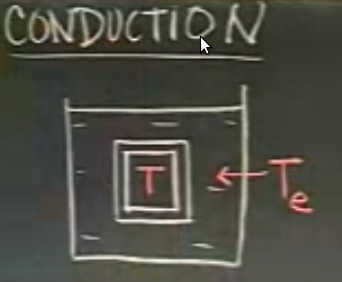
\includegraphics[height=4cm]{3_1.png}

Newton'un Soguma Kanununu kullaniyoruz ve sicakligin aktarilarak baska
bir noktaya gectigini dusunuyoruz (sicaklik radyasyon uzerinden de
seyahat edebilir), ve su modeli kuruyoruz. 

\[ \frac{dT}{dt} = k(T_e - T) \]

$k > 0$ akiskanlik (conductivity), bir sabit.

\[ T(0) = T_0 \]

$T$'nin zamana gore bir fonksiyon oldugunu unutmayalim. Kisa olsun diye
cogu zaman $T(t)$ ibaresi kullanilmiyor. 

Yayilma (diffusion) modeli nasil olurdu? 

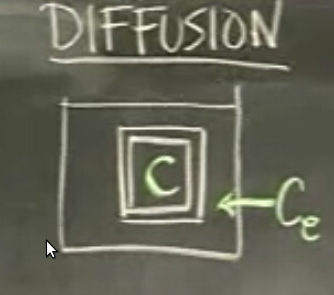
\includegraphics[height=4cm]{3_2.png}

Bu model formulsel olarak neredeyse ayni, diyelim ki bu sefer kup
icinde tuz var, konsantrasyonu $C$, disaridaki tuz kontsantrasyonu
$C_e$. Yayilma modelinde tuzluluk ``yayiliyor'', yuksek konstrasyondan
alcak olana dogru gidiyor. Bu modelde tuzun yayilma hizi,
konstantrasyonlar arasindaki farka baglidir. 

\[ \frac{dC}{dt} = k(C_e - C) \]

Isi aktarim formulu standart lineer formda degil, bu degisimi
yapalim, ki en azindan lineer oldugunu gormus olalim. 

\[ \frac{dT}{dt} + kT = kT_e \]

Cozelim

\[ y' + p(x)y = q(x) \]

Bu formulu entegre edici faktor (integrating factor) $u(x)$ kullanarak
cozecegiz.

\[ uy' + puy = qu \]

Burada yapmak istedigimiz oyle bir $u$ bulmak ki sag ve sol taraf
onunla carpilinca sol taraf bir seyin turevi haline gelsin:

\[ ( ... )' = ..  \]

Boylece $x$'e gore iki tarafin entegralini alinca turev islemi
kaybolur, daha temiz bir ifade geriye kalir. 

Parantez icinde ulasmaya calisacagimiz ifade neye benzemeli? Hoca
$(uy)'$ fikrini ortaya atti. Bunun niye mantikli bir secim oldugunu
gormek zor degil, eger $(uy)'$ uzerinde turevin carpim kuralini
kullanirsak, acilimi zaten 

\[ uy' + u'y \]

olacaktir, ki bu ifade $uy' + puy = qu$ formulunun sol tarafina
yakindir. Tek bir farkla, $u'$ yerine elimizde $pu$ var. O zaman u
oyle secilmeli ki $u' = pu$ olsun. 

\[ u' = pu \]

Degiskenleri ayir

\[ \frac{du}{u} = p \]

Entegrali al

\[ \int \frac{du}{u}  = \int p \]

\[ ln (u) = \int p(x) dx \]

Buradan $u$'nun ne olacagini kestirebiliriz. Unutmayalim, tum $u$'lara
ihtiyacim yok, ustteki ifadeyi tatmin eden herhangi bir $u$
olabilir. Ustteki formulun iki tarafina $e$ bazina tabi tutarsak

\[ u = e^{\int p(x) dx} \]

Iste entegre edici faktoru bulduk. Rasgele (arbitrary) sabite ihtiyac
yok cunku tek $u$ kullandik.

Metotu tekrar bastan gozen gecirelim. Elimizde su var:

\[ y'+py = q \]

1. Eger formul standart lineer formda degilse o forma gecir, cunku
entegre edici formulde $p$ var, eger form dogru degilse dogru $p$
gelmez, isler sarpa sarar.

2. Entegre edici faktoru \[ e^{\int p(x) dx} \] bul.

3. ODE'nin iki tarafini bu faktor ile carp.

4. Entegre et

Ornek

\[ xy' - y= x^3 \]

Standart form

\[ y' - \frac{1}{x}y = x^2 \]

Entegre edici faktor

\[ e^{-ln(x)} \]

Bunu daha basitlestirebiliriz,

\[ e^{-ln(x)} = (e^{ln(x)})^{-1} = x^{-1} = \frac{1}{x}  \]

Standart formun iki tarafini bu faktor ile carpalim

\[ \frac{1}{x}y' - \frac{1}{x^2}y = x \]

Eger her seyi dogru yaptiysak sol tarafi direk entegre
edebiliriz. Parantezli forma koyalim, ve parantez icinin hakikaten
ustteki sonucu verip vermedigine de dikkat edelim.

\[ (\frac{1}{x}y)' = x \]

Entegrali alinca

\[ \frac{1}{x}y = \frac{x^2}{2} + C \]

\[ y = \frac{x^3}{2} + C \]

Sonucu bulduk.

Ornek 

\[ (1+cos(x))y' - (sin(x))y = 2x \]

\[ y' = \frac{sin(x)}{1+cos(x)}y = \frac{2x}{1+cos(x)} \]

Ent. edici faktor

\[ - \int \frac{sin(x)}{1+cos(x)} dx \]

Bu bayagi korkutucu bir entegral gibi gozukuyor. Fakat dikkatli
bakarsak bolumun ust tarafi alt tarafinin turevi. Bu cok iyi, o zaman
entegrasyon su sonucu verir:

\[ ln (1+cos(x)) \]

Faktor ise

\[ e^{ln (1+cos(x))} = 1+cos(x) \]

Iki tarafi faktor ile carpalim

\[ (1+\cos(x)) y' - \sin(x)y = 2x \]

Burada ilginc bir durum var, bu sonuc ornegin ta kendisi! Buradan
anliyoruz ki ODE daha bastan beri parantez icinde gruplanabilir bir
haldeymis. Yani

\[ [(1+cos(x))y]' = 2x \]

Iki tarafin entegralini alalim

\[ (1+cos(x))y = x^2 \]

\[ y = \frac{x^2+C}{1+cos(x)} \]

Diyelim ki problem bize bir baslangic sarti, $y(0) = 1$ verdi. O zaman

\[ 1=\frac{c}{2}, c=2 \]

Bunu $y$ formulune koyarsak cozumu tamamlamis oluruz. 

k Tane Sabit Iceren Lineer ODE

Bu formda $p(x)$ bir sabit olacak, bu sabitli form oldukca onemli,
banka hesaplari vs. gibi pek cok modelde karsimiza cikiyor.

\[ \frac{dT}{dt} + kT = kT_e \]

Faktor? k'nin entegrali nedir? $\int k dt = kt$. O zaman

\[ e^{kt} \]

Iki tarafi bununla carpalim. 

\[ (e^{kt} T)' = kT_e e^{kt} \]

Iki tarafin entegralini alalim

\[ e^{kt} T = \int kT_e(t) e^{kt}dt + C\]

\[ T = e^{-kt} \int kT_e(t) e^{kt} dt + C e^{-kt} \]

Cogu insan, cogunlukla muhendislik literaturunde, ustteki cozumu
tanimsiz (indefinite) entegral halinde birakmayi sevmez, cunku
tanimsiz entegral .. tanimsizdir; baska bir deyisle tanimsiz bir
entegral bir degil pek cok mumkun fonksiyonlari ayni anda temsil eder,
ve bu tum mumkun fonksiyonlarin arasindaki fark sonsuz tane farkli
olabilecek sabit sayidir (bu yuzden zaten baslangic sartini alarak
somut bir $C$ degeri bulmaya calisiriz). 

Bu tur literaturde eger bir baslangic sarti var ise, mesela $T(0) =
T_0$ gibi, 
bu kisiler tanimsiz entegrali su sekilde tanimli hale getirmeyi seviyorlar. 

\[ T = e^{-kt} \int_0^t kT_e(t_1) e^{kt_1} dt_1 + C e^{-kt} \]

Yani alt sinir olarak sifir, ust sinir olarak $t$ aliniyor. Yeni bir
$t_1$ degiskeni koyulur, bu bir fuzuli (dummy) bir degiskendir, sadece
yer tutmasi icin oraya konur. Bu neyi saglar? Zaman $t=0$ oldugunda ne
olduguna bakalim, o zaman toplamin sol tarafi tamamen yokoluyor,
geriye sadece $C = T_0$ kaliyor, boylece hem $C$ degerini $T_0$ olarak
kullanabilmis oluruz, hem de tanimsiz entegrali tanimli hale getirmis
oluruz. 

Peki $t$ sonsuza giderken, yani cok zaman gectikce, bu sisteme ne
olur? $k > 0$ sartini unutmayalim, sonsuza gidilirken bu sefer
toplamin sag tarafi sifira gider. Cunku eksi degerli bir ustel deger
$k$ hep arti kalacagina gore buyudukce $e$ degerini sifira
goturur. Bu sistemin istikrarli konum (steady state) cozumu sudur.

\[ T = e^{-kt} \int_0^t kT_e(t_1) e^{kt_1} dt_1 \]

Sifira giden kisim ``gecici'' bolum olarak adlandirilir. 

Bu bize bir sey daha soyluyor. Sonsuza giderken sifira giden bolumde
baslangic sarti vardi. Demek ki baslangic sartinin uzun zaman
gectikcen sonra varilacak nokta konusunda hicbir onemi, etkisi
yoktur. Nereden baslarsak baslayalim, bir sure sonra ayni noktaya
variriz. 

\end{document}
